\usetikzlibrary{shapes, arrows}
\usetikzlibrary{positioning}
\usetikzlibrary{shapes.geometric, arrows, positioning}
\usetikzlibrary{intersections, patterns, calc}

\tikzstyle{startstop} = [rectangle, rounded corners, minimum width=2cm, minimum height=1cm, text centered, draw=black]
\tikzstyle{process} = [rectangle, minimum width=2cm, minimum height=1cm, text centered, draw=black]
\tikzstyle{decision} = [diamond, minimum width=2cm, minimum height=1cm, text centered, draw=black]
\tikzstyle{arrow} = [thick,->,>=stealth]

\chapter{Generowanie modeli PL z~opisów tekstowych zagadnień optymalizacyjnych}\label{ch:generation}

\section{Model Programowania Liniowego}
% - Model Programowania Liniowego - tutaj definicja, która jest zgodna z reprezentacją ZIMPL
\subsection{Definicja}
\textbf{Zbiór \boldmath$S$.} 
Niech $S$ będzie zbiorem, którego elementami są inne zbiory lub wektory zbiorów. Każdy taki element może zawierać liczby, ciągi znakowe (tekstu) albo krotki składające się z liczb i ciągów tekstowych. Jeżeli pewien $S \in S$ jest wektorem, wówczas jego wymiary (indeksy) są określane przez wartości innego zbioru $S' \in S \setminus \{S\}$.

\medskip
\textbf{Zbiór \boldmath$P$.}
Niech $P$ będzie zbiorem parametrów. Każdy parametr $p \in P$ może być pojedynczą liczbą albo wektorem liczb indeksowanym poprzez wartości jakiegoś zbioru z~$S$.

\medskip
\textbf{Zbiór \boldmath$V$.}
Niech $V$ będzie zbiorem zmiennych. Każda zmienna $v \in V$ może występować jako pojedyncza zmienna bądź wektor zmiennych, indeksowany przez wartości z~odpowiedniego zbioru w~$S$. Dodatkowo dziedzina każdej zmiennej jest ciągła bądź całkowitoliczbowa, a ponadto ograniczona skończonymi wartościami od dołu i~od góry. Granice te można wyrażać za pomocą parametrów z~$P$.

\medskip
\textbf{Funkcja celu \boldmath$f(S,P,V)$.}
Funkcja $f(S,P,V)$ jest liniowa względem zmiennych z~$V$ i~może (opcjonalnie) korzystać z~parametrów z~$P$, jak również z~dowolnych wyrażeń algebraicznych związanych ze zbiorami z~$S$.

\medskip
\textbf{Zbiór ograniczeń \boldmath$G$.}
Niech $G$ będzie zbiorem ograniczeń. Każde ograniczenie ma postać
\[
g(S,P,V) \;\leq\; 0,
\]
gdzie $g$ jest funkcją liniową w~zmiennych $V$, przy czym może używać parametrów $P$ i~wyrażeń odnoszących się do zbiorów z~$S$.

\medskip
\textbf{Model \textit{PL}.}
Model programowania liniowego (\textit{PL}) definiujemy jako krotkę
\[
M \;=\; (\,S,\,P,\,V,\,f,\,G\,).
\]
\subsection{Przykładowy model \akronim{PL} w języku \akronim{ZIMPL} dla problemu optymalnego doboru ilościowego dwóch rodzajów żywności}
\begin{lstlisting}[language=zimpl]
set Foods := {"FoodI", "FoodII"};
set Vitamins := {"VitaminA", "VitaminC"};

# Parameters for costs
param cost[Foods] := 
    <"FoodI"> 5, 
    <"FoodII"> 7;

# Parameters for vitamin limits
param vitamin_limit[Vitamins] := 
    <"VitaminA"> 8, 
    <"VitaminC"> 10;

# Vitamin content per food (matrix representation)
param content[Foods * Vitamins] :=
             | "VitaminA", "VitaminC" |
|"FoodI"     |          2,          1 |
|"FoodII"    |          1,          2 |;

# Decision variables: amount of each food (in kg)
var x[<f> in Foods] >= 0;

# Objective function: Minimize the total cost
minimize total_cost: sum <f> in Foods: cost[f] * x[f];

# Constraints: Ensure vitamin requirements are met
subto vitamin_constraints: 
    forall <v> in Vitamins do
        sum <f> in Foods: content[f,v] * x[f] >= vitamin_limit[v];

\end{lstlisting}
\subsection*{Krotka \boldmath$M = (S, P, V, f, G)$}

\begin{enumerate}
  \item \textbf{Zbiory} (\boldmath$S$)
  \begin{itemize}
    \item $S = \{\text{Foods},\, \text{Vitamins}\}$, gdzie:
    \begin{itemize}
      \item $\text{Foods} = \{\text{'FoodI'}, \text{'FoodII'}\}$ -- zbiór rodzajów żywności,
      \item $\text{Vitamins} = \{\text{'VitaminA'}, \text{'VitaminC'}\}$ -- zbiór wymaganych witamin.
    \end{itemize}
  \end{itemize}

  \item \textbf{Parametry} (\boldmath$P$)
  \begin{itemize}
    \item $P = \{\text{cost},\, \text{vitamin\_limit},\, \text{content}\}$, gdzie:
    \begin{itemize}
      \item $\text{cost}[f]$: koszt jednostkowy żywności $f \in \text{Foods}$ \\
            (np. $\text{cost}[\text{'FoodI'}] = 5$),
      \item $\text{vitamin\_limit}[v]$: minimalna wymagana ilość witaminy $v \in \text{Vitamins}$ \\
            (np. $\text{vitamin\_limit}[\text{'VitaminA'}] = 8$),
      \item $\text{content}[f,v]$: zawartość witaminy $v$ w~1\,kg żywności $f$ \\
            (np. $\text{content}[\text{'FoodI'}, \text{'VitaminA'}] = 2$).
    \end{itemize}
  \end{itemize}

  \item \textbf{Zmienne decyzyjne} (\boldmath$V$)
  \begin{itemize}
    \item $V = \{\,x\,\}$, gdzie $x$ to wektor indeksowany przez $\text{Foods}$:
    \[
      x[f] \;\geq\; 0 \quad\text{dla}\; f \in \text{Foods}.
    \]
    Interpretacja: $x[f]$ oznacza ilość (w~kg) żywności $f$ w~mieszance (zmienna nieujemna, ciągła).
  \end{itemize}

  \item \textbf{Funkcja celu} (\boldmath$f$)
  \begin{itemize}
    \item Definiujemy:
    \[
      f(S,P,V) \;=\; \sum_{f \in \text{Foods}} \text{cost}[f] \cdot x[f].
    \]
    Celem jest minimalizacja łącznego kosztu mieszanki:
    \[
      \min \quad \sum_{f \in \text{Foods}} \text{cost}[f] \cdot x[f].
    \]
  \end{itemize}

  \item \textbf{Zbiór ograniczeń} (\boldmath$G$)
  \begin{itemize}
    \item Dla każdej witaminy $v \in \text{Vitamins}$ wymagamy:
    \[
      \sum_{f \in \text{Foods}} \text{content}[f,v] \cdot x[f]
      \;\;\geq\;\;
      \text{vitamin\_limit}[v].
    \]
    \medskip
    Aby sprowadzić nierówność do postaci $\leq 0$ (zgodnie z~Definicją~3.1.1):
    \[
      - \sum_{f \in \text{Foods}} \text{content}[f,v] \cdot x[f]
      \;+\;
      \text{vitamin\_limit}[v]
      \;\;\leq\;\; 0.
    \]
    \end{itemize}
\end{enumerate}

\section{Problem generowania modelu PL z opisu tekstowego}
% - Problem generowania modelu PL z opisu tekstowego - tutaj poza formalnym postawieniem problemu należy omówić właściwości tego problemu; zdefiniujcie też warianty problem z parametryzacją i bez parametryzacji - tutaj mamy opisac ktore fragmenty kodu oraz w jaki sposob tworza model w zimpl? jesli tak to jest to w rozdziale 4.1.2



\section{Problem oceny modelu PL na zgodność z opisem tekstowym}
% -  - formalny opis problemu i jego właściwości - powinnismy przedstawic jakie kategorie oceny wybralismy? Pytanie rowniez czym jest formalny opis problemu


% TP: Po co to? Przecież nie rozwiązujecie modeli PL, ani nie korzystacie w żaden sposób z tych twierdzeń; one też nie pasują do ogólniejszej klasy -> MILP, którą Wasza metoda obsługuje

% TP: TODO: Tutaj też sugeruję nie rozwodzić się nad zapisami, które są istotne z punktu widzenia metod rozwiązywania modeli PL; z punktu widzenia modelowania rozróżnienie postaci ogólnej i standardowej nie ma większego znaczenia. Z drugiej strony brakuje definicji modelu PL takiego, który Wy generujecie. 
% Dlatego sugeruję tutaj wprowadzić 3 sekcje:
% - Model Programowania Liniowego - tutaj definicja, która jest zgodna z reprezentacją ZIMPL
% - Problem generowania modelu PL z opisu tekstowego - tutaj poza formalnym postawieniem problemu należy omówić właściwości tego problemu; zdefiniujcie też warianty problem z parametryzacją i bez parametryzacji
% - Problem oceny modelu PL na zgodność z opisem tekstowym - formalny opis problemu i jego właściwości
% W załączeniu do maila dołączam przykładową pracę mgr, w której autor definiuje model PL i problem odkrywania modelu PL z danych (rozdział 2). Możecie się zasugerować, ale proszę nie przepisywać żywcem bo to byłby plagiat!




\section{Propozycja rozwiązania}

% TP: TODO: bardzo proszę trzymać się nazewnictwa:
% - "zagadnienie" to zagadnienie optymalizacyjne
% - "problem" to problem odkrywania modelu PL lub problem ocen modelu PL
% - "rozwiązanie" to rozwiązanie modelu PL
% TP: Nie używajcie modyfikatora [H] do figure; niech latex to sam ułoży wg ogólnych zasad.

% TP: TODO: Sugeruję takie sekcje:
% - Architektura systemu - tutaj należy dorobić rysunek architektury i odpowiednio dostosować poniższy opis; w opisie rozdzielcie architekturę od przepływu sterowania. Powinny być osobno omówione dwa przepływy sterowania: generowanie modelu i ocena modelu. Tutaj też odwołajcie się do zbioru danych i napiszcie, że jest on dokładnie omówiony w rozdziale \ref{ch:dataset}. Gdzieś tutaj powinno pojawić się też odniesienie do usług OpenAI, które wykorzystaliście.
% Adam - mozesz Jagoda napisac o tych uslugach
% - Inżynieria podpowiedzi - tutaj opiszcie jak powstały prompty używane w poszczególnych problemach, jak były testowane i rozwijane; - DONE w rozdziale 3.5


% jeśli są dostępne jakieś wyniki eksperymentalne krótko (np. na jednym wykresie) pokazujące poprawę jakości uzyskiwanych wyników dla kolejnych wersji to też możecie pokazać; Na koniec jako listing kodu możecie pokazać wynikowe prompty, być może mniejszą czcionką. 
% Te opisy też powinny być bardziej konkretne i zwięzłe. Trzeba napisać np. jak nauczyliście DMJ ZIMPLa.
% Adam: Masz może te wykresy Jagoda? Możesz też wstawić wynikowe prompty. 


\begin{figure}
    \centering
    \begin{tikzpicture}[node distance=1.5cm]
    
    % Nodes
    \node (input) [startstop] {Para: \textit{problem -- kod modelu}};
    \node (template) [process, below=1cm of input] {Szablon zapytania};
    \node (dmj1) [cloud, draw, below=0.75cm of template] {\textbf{DMJ}};
    \node (validator) [process, below=0.75cm of dmj1] {Walidacja działania kodu};
    \node (dmj2) [cloud, draw, below=0.75cm of validator] {\textbf{DMJ}};
    \node (evaluation) [process, below=0.75cm of dmj2] {Ocena jakości modelu};
    \node (solution) [startstop, below=1cm of evaluation] {Rozwiązanie optymalne};
    \node (experts) [process, right=4cm of validator] {Eksperci};
    
    % Arrows
    \draw [arrow] (input) -- (template);
    \draw [arrow] (template) -- (dmj1);
    \draw [arrow] (dmj1) -- (validator);
    \draw [arrow] (validator) -- (dmj2);
    \draw [arrow] (dmj2) -- (evaluation);
    \draw [arrow] (evaluation) -- (solution);
    \draw [arrow, dashed] (validator.east) -- node[midway, above] {Wystąpienie błędu} (experts.west);
    \draw [arrow, dashed] (experts.north) to[out=90,in=0] (template.east);
    \draw [arrow, dashed] (evaluation.east) to[out=0,in=270] node[midway, above, fill=white] {Rozwiązanie niesatysfakcjonujące} (experts.south);



    \end{tikzpicture}

\caption{Schemat walidacji kodu modelu}
\label{fig:workflow}
\end{figure}

Wizualny opis rozwiązania został przedstawiony na rysunku \ref{fig:workflow}. % TP: łatwiej jest zrozumieć, kiedy od początku jest odwołanie do schematu
Rozwiązanie rozpoczyna się od utworzenia bazy danych z parami: \textit{problem} jako opis słowny problemu \textit{PL} oraz \textit{kod modelu} jako poprawny kod w języku \textit{ZIMPL}. Następnie tworzony jest \textit{Szablon zapytania}, który wykorzystuje schemat zaczerpnięty z materiałów edukacyjnych opisanych w dziale \ref{sec:model_example}. \textit{Szablon zapytania} kierowany jest do \textit{DMJ} w celu generacji modelu \textit{PL}. W związku z niskim kosztem i pozytywnymi wynikami, do tworzenia zapytania wykorzystano model \texttt{GPT 4o-mini}. Wygenerowany \textit{model} zostaje poddany procesowi \textit{Walidacji działania kodu}, korzystając z programu \href{https://www.scipopt.org/}{SCIP} \cite{BolusaniEtal2024ZR}. % TP: TODO: SCIP ma oficjalną publikację do cytowania https://www.scipopt.org/index.php#cite - DONE

 Zdecydowano się na \textit{SCIP}, ponieważ jest to darmowe, otwarte oprogramowanie z rozbudowaną dokumentacją. % TP: TODO <- unikajcie niepotwierdzonych stwierdzeń; prawdopodobnie można znależć benchmarki, w których SCIP wypada słabiej od konkurencji; wybór SCIPa wynika z jego dostępności; to jest projekt open-source - DONE
 W przypadku wystąpienia błędu w wygenerowanym kodzie, program do \textit{Walidacji działania kodu} powiadamia o tym \textit{Ekspertów}, którzy przystępują do rekonstrukcji szablonu zapytania.

Jeśli \textit{Walidacja działania kodu} zakończy się sukcesem, wygenerowany kod jest oceniany poprzez niezależny \textit{DMJ}. Aby uniknąć sytuacji, w której model oceniający jest taki sam jak model generujący kod, zdecydowano się na wykorzystanie modelu \texttt{GPT-4} do ewaluacji działania generatora. Jeśli \textit{Ocena jakości modelu} zwróci \textit{niesatysfakcjonujące rozwiązanie} jest ono zwracane do \textit{Ekspertów} w celu refaktoryzacji \textit{Szablonu zapytania}. Modele wynikowe \textit{ZIMPL} oraz walidator punktujący poszczególne zadania są poddawane sprawdzeniu i czyszczeniu z ewentualnych nieścisłości wywołanych przez halucynacje \textit{DMJ}, poprzez usuwanie i modyfikację częstych błędów.


% \textbf{TODO - dodaje opis zbioru treningowego do przerobienia}
% Jagoda: Dodaje akapit do wrzucenia do rozdziału 3 (tego co uważacie za słuszne)
% TP: TODO: poniższy akapit jest w zasadzie o inżynierii podpowiedzi i jako taki bardziej pasuje do opisu metody (Rozdział 3) niż zbioru danych - DONE

Nie każdy przykład ze zbioru został wykorzystany we wszystkich zapytaniach. W związku ze specyfiką tworzonego kodu, zapytania zostały podzielone na kategorie: programowanie sztywne i programowanie z parametryzacją. Następnie utworzono trzy zapytania, każde odpowiadające określonej części definicji problemu, na które składają się: zmienne decyzyjne, funkcja celu oraz ograniczenia. Do każdego z trzech różnych zapytań dotyczących programowania sztywnego % TP: TODO <- Nie wiadomo skąd się bierze liczba 4, dlaczego akurat tyle i jak te zapytania są wybierane - Jagoda: w przypadku sztywnego kodowania wysyłane są 4 zapytania, warto to uwzględnić w opisie w rozdziale 3 % Adam x2 - sa 3 DONE
dodano wszystkie wybrane opisy zadania programowania liniowego
wraz z elementem kodu  \akronim{ZIMPL}, którego dotyczy zapytanie. Łącznie uwzględniono 10 takich zapytań. Podobnie zrealizowano zadanie dla programowania z parametryzacją. Utworzono pięć różnych zapytań, po jednym na każdą część definicji problemu: zestawy danych, parametry, zmienne decyzyjne, funkcja celu, ograniczenia. Dla każdego z pięciu zapytań, wykorzystano 10 zadań wraz z elementami kodu  \akronim{ZIMPL}. % TP: TODO <- dlaczego 6 i jak zostały wybrane? - Jagoda: tutaj podobnie dla parametryzowanego wysyłamy 6 zapytań, warto dopisac w rodziale % Adam x2 - DONE


\section{Inżynieria podpowiedzi}
% - Inżynieria podpowiedzi - np. na podstawie https://pl.wikipedia.org/wiki/Inżynieria_podpowiedzi
Inżynieria podpowiedzi (ang. \textit{prompt engineering}) to proces projektowania i iteracyjnego doskonalenia instrukcji przekazywanych \textit{DMJ} w celu uzyskania satysfakcjonujących wyników. Poprawnie zaprojektowane podpowiedzi mogą znacząco wpłynąć na jakość generowanych wyników, szczególnie w kontekście złożonych modeli \textit{PL}.

W niniejszej pracy inżynieria podpowiedzi została zastosowana do automatycznego generowania modeli \textit{PL} w języku \textit{ZIMPL}. Proces ten polegał na iteracyjnym dostosowywaniu treści podpowiedzi na podstawie wyników uzyskanych w poprzednich iteracjach. Pozwoliło to usprawnić proces generowania modeli \textit{PL} oraz poprawa ich jakości.

W pracy wykorzystano inżynierie podpowiedzi, której kroki opisano poniżej:
\begin{itemize} 
\item Model językowy (\textit{DMJ}) generuje model \textit{PL} w języku \textit{ZIMPL} na podstawie opisu problemu w języku naturalnym. 
\item Wygenerowany model jest oceniany przez niezależny moduł lub specjalistę. Ocena opiera się na: 
    \begin{itemize} 
        \item zgodności wyników z wymaganiami i specyfikacją problemu, 
        \item porównaniu z ręcznie opracowaną wersją kodu, która służy jako punkt odniesienia. 
    \end{itemize} 
\item Na podstawie tej analizy, instrukcje generacji są modyfikowane i dostosowywane, aby poprawić jakość wyników w kolejnych iteracjach.\end{itemize}


\section{Graficzny interfejs użytkownika}\label{sec:generation:gui}

%Zakładając możliwość komercyjnego wykorzystania generatora modeli, s
Stworzono interfejs graficzny wykorzystując narzędzie \textit{Streamlit} \cite{Streamlit2019} oraz gotowy przepływ zapytań \textit{DML} \cite{TODO}. Jako funkcjonalności narzędzia można wyróżnić:

\begin{enumerate}
\item Rozwijany pasek boczny z zapisaną historią poprzednich rozwiązań wygenerowanych w czasie sesji oraz możliwością edycji i usuwania.
\item Przycisk wyboru formatu generowanego modelu \textit{ZIMPL}: z parametryzacją lub bez parametryzacji.
\item Obszar do wpisywania i edycji zapytań.
\item Przycisk generowania modelu \textit{ZIMPL}.
\item Obszar wypisywania wygenerowanych wyników z możliwością edycji.
\end{enumerate}

\begin{figure}[H]
\centering
\begin{tikzpicture}[
    app/.style={draw, thick, rectangle, rounded corners, minimum width=\textwidth, minimum height=14cm, fill=gray!10},
    largebox/.style={draw, thick, rectangle, rounded corners, fill=white, minimum height=4cm, minimum width=0.55\textwidth, anchor=north east},
    smallbox/.style={draw, thick, rectangle, rounded corners, fill=white, align=center, minimum height=1cm, minimum width=4cm, anchor=center},
    dropdown/.style={draw, thick, rectangle, rounded corners, fill=white, align=center, minimum height=9cm, minimum width=0.35\textwidth, anchor=north west},
    text/.style={font=\small}
]

\node[app] (app) {};

\node[dropdown, xshift=0.5cm, yshift=-1cm] (dropdown) at ([yshift=-1cm]app.north west) {Pasek rozwijany: \\ \textit{Historia rozwiązań}};
\node[largebox, xshift=-0.5cm, yshift=-1cm] (inputArea) at ([yshift=-1cm]app.north east) {\centering{Pole tekstowe: \parbox{5cm}{\textit{Opis problemu}}}};
\node[smallbox, yshift=1cm] at (inputArea.north) {Przycisk: Zmiana parametryzacji};
\node[smallbox, below=0.8cm of inputArea.south] (generateButton) {Przycisk: Generuj kod};
\node[largebox, below=0.8cm of generateButton] (resultArea) {\centering{Pole tekstowe: \parbox{5cm}{\textit{Wynik wygenerowanego kodu}}}};
\node[smallbox, below=0.8cm of dropdown.south] (deleteButton) {Przycisk: Usuń rozwiązanie};

\end{tikzpicture}
\caption{Schemat graficzny interfejsu aplikacji z opisem elementów.}
\label{fig:application-diagram}
\end{figure}

Na Rysunku \ref{fig:application-diagram} przedstawiono wizualizację ekranu generatora wraz z układem jego funkcjonalności. Poniżej znajduje się obraz \ref{fig:gui} zrzutu ekranu interfejsu użytkownika.

% TP: TODO: dla kompletności pokażcie też zrzut ekranu z GUI - DONE

\begin{figure}[H]
    \centering
    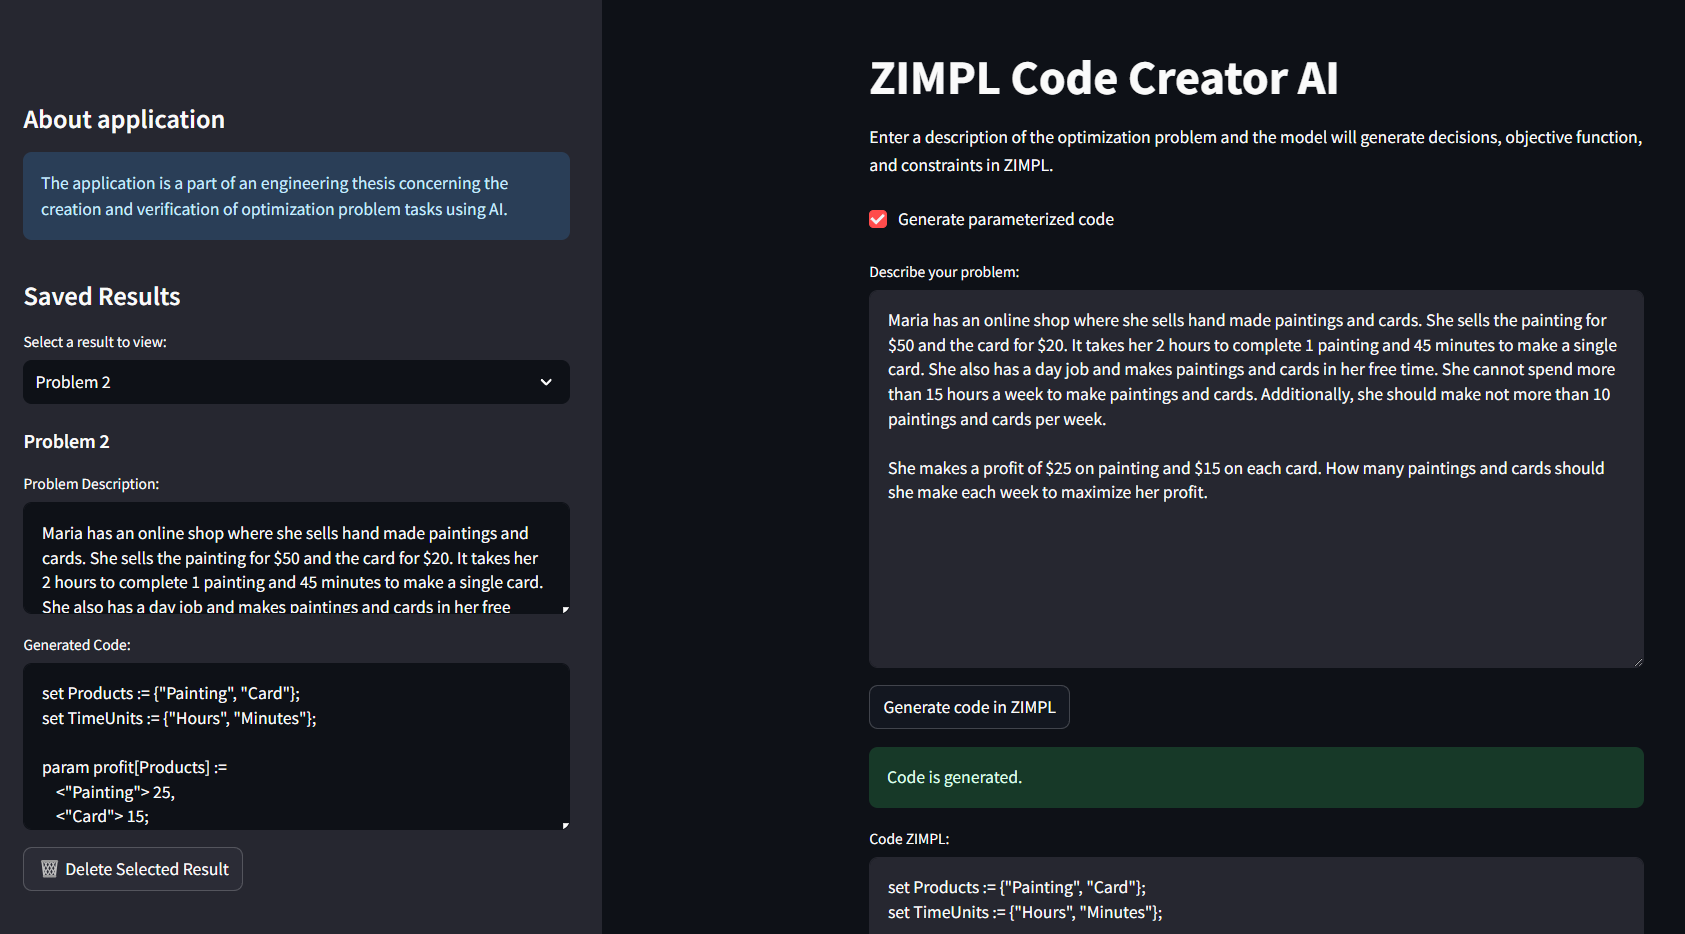
\includegraphics[width=1\linewidth]{figures\\app.png}
    \caption{Wygląd interfejsu generatora kodu ZIMPL}
    \label{fig:gui}
\end{figure}





